\chapter{实验测试与分析}

本节使用的 InSAR 测试数据是 GMTSAR 官方提供的2010年4月下加利福尼亚州 $7.2 M_w$ 地震前后的 ALOS 卫星数据。主、副 SAR SLC 图像分别拍摄于2009年12月17日和2010年5月4日。SLC 图像大小为一个标准的 ALOS 图像帧,方位向和距离向长度各为 27648 像素和 11304 像素。软件测试环境如表 \ref{tab:env} 所示。

\begin{table}[htbp]
\centering
\begin{tabular}{|l|l|l|}
\hline
    \multirow{3}{*}{CPU}                        & 型号     & Intel Xeon E5-2650 v4                 \\ \cline{2-3} 
                                                & 核心数   & $\times 12$                           \\ \cline{2-3} 
                                                & 主频     & 2.20 GHz                              \\ \hline
    \multicolumn{2}{|l|}{内存}                             & 32768 MiB                             \\ \hline
    \multicolumn{2}{|l|}{操作系统}                         & Ubuntu 16.04.2 LTS, Linux 4.4.0 内核  \\ \hline
    \multicolumn{1}{|c|}{\multirow{2}{*}{编译}} & 编译器   & gcc 5.4.0                             \\ \cline{2-3} 
    \multicolumn{1}{|c|}{}                      & 编译参数 & \texttt{-O2 -march=native}            \\ \hline
\end{tabular}
\caption{软件测试环境} \label{tab:env}
\end{table}

\section{图像拼接算法测试}

并行图像拼接算法的实验测试中,因为数据来源有限,仅仅使用了6个同一轨道号的连续的 SAR 图像帧进行测试。图 \ref{fig:exp_merge} 展示了并行线程数对拼接程序性能的影响。可以看到,并行归约算法将拼接时间缩短了一半以上。比较遗憾的是,由于要拼接的图像帧数量较少,归约算法的线程数很快就收敛了,并行算法性能大概在2~3个线程时就达到了饱和。

\begin{figure}[htbp]
\centering
\subfloat[程序计算时间]{
    \label{fig:exp_merge_a}
    \begin{minipage}[t]{0.49\textwidth}
        \centering
        \resizebox {\textwidth} {!} {
            \begin{tikzpicture}
\begin{axis}[
    xlabel={并行线程数},
    ylabel={计算时间/s},
    xmin=1, xmax=7,
    ymin=0, ymax=200,
    xtick={1, 2, 3, 4, 5, 6, 7},
%    ytick={ },
    legend pos=north east,
    ymajorgrids=true,
    grid style=dashed,
]

\addplot[
    color=red,
    mark=square,
    style=solid,
    ]
    coordinates {
        (1, 194.972254756)
        (2, 106.441216719)
        (3, 91.799094679)
        (4, 92.142388643)
        (5, 92.000214744)
        (6, 88.829891908)
        (7, 83.641275544)
    };
\end{axis}
\end{tikzpicture}

        }
    \end{minipage}
}
\subfloat[CPU 核心利用率]{
    \label{fig:exp_merge_b}
    \begin{minipage}[t]{0.49\textwidth}
        \centering
        \resizebox {\textwidth} {!} {
            \begin{tikzpicture}
\begin{axis}[
    xlabel={并行线程数},
    ylabel={CPU 核心占用},
    xmin=1, xmax=7,
    ymin=0, ymax=4,
    xtick={1, 2, 3, 4, 5, 6, 7},
%    ytick={ },
    legend pos=north east,
    ymajorgrids=true,
    grid style=dashed,
]

\addplot[
    color=red,
    mark=square,
    style=solid,
    ]
    coordinates {
        (1, 1.000)
        (2, 1.862)
        (3, 2.257)
        (4, 2.258)
        (5, 2.298)
        (6, 2.425)
        (7, 2.575)
    };
\end{axis}
\end{tikzpicture}

        }
    \end{minipage}
}
\caption{线程数对 SAR 图像帧并行拼接算法性能的影响} \label{fig:exp_merge}
\note{\small 测试数据共6个 ALOS 图像帧}
\end{figure}
 
该例子说明,并行算法的性能并非总是随着线程数的增加而提升。计算线程数量超过一定值后,多余的线程将不会改善程序性能,必须改进算法或者提高数据量以增加可利用的线程数。此外,线程数量增加时,线程间通信的成本会增加,其他不可并行资源访问(如磁盘读写)也可能达到性能瓶颈。

图像拼接算法完全是确定性的,不会受拼接顺序影响。经过验证。并行拼接与顺序拼接的结果完全一致。

\section{图像配准算法测试}

图 \ref{fig:exp_cores} 展示了默认计算参数(见表 \ref{tab:xcorr-args})下 xcorr2 性能随计算线程数的变化趋势。当计算线程从无增加至6个时,图 \ref{fig:exp_cores_a} 显示的计算时间缩短非常显著。但当计算线程数进一步增加时,运行时间并没有显著变化。图 \ref{fig:exp_cores_b} 中的 CPU 核心使用率也反应了这种趋势,当计算线程数多于6个时,核心使用率少于计算线程数,说明程序已经无法充分利用所有的 CPU 核心。后面的实验中将使用8个计算线程对 xcorr2 并行性能进行评估,

\begin{figure}[htbp]
\centering
\subfloat[程序计算时间]{
    \label{fig:exp_cores_a}
    \begin{minipage}[t]{0.49\textwidth}
        \centering
        \resizebox {\textwidth} {!} {
            \begin{tikzpicture}
\begin{axis}[
    xlabel={计算线程数},
    ylabel={计算时间/s},
    xmin=0, xmax=12.2,
    ymin=0, ymax=12,
    xtick={0, 2, 4, 6, 8, 10, 12},
%    ytick={ },
    legend pos=north east,
    ymajorgrids=true,
    grid style=dashed,
]
\addplot[
    color=blue,
    mark=square,
    ]
    coordinates {
        (0, 11.200907922)
        (1, 10.521500231)
        (2, 5.431319614)
        (3, 3.757715043)
        (4, 2.918596810)
        (6, 2.146015373)
        (8, 2.052885075)
        (12, 2.181156634)
    };
    \legend{xcorr2} 
\end{axis}
\end{tikzpicture}

        }
    \end{minipage}
}
\subfloat[CPU 核心利用率]{
    \label{fig:exp_cores_b}
    \begin{minipage}[t]{0.49\textwidth}
        \centering
        \resizebox {\textwidth} {!} {
            \begin{tikzpicture}
\begin{axis}[
    xlabel={计算线程数},
    ylabel={占用 CPU 核心数},
    xmin=0, xmax=12.2,
    ymin=0, ymax=10,
    xtick={0, 2, 4, 6, 8, 10, 12},
%    ytick={ },
    legend pos=north west,
    ymajorgrids=true,
    grid style=dashed,
]

\addplot[
    color=red,
    mark=square,
    style=solid,
    ]
    coordinates {
        (12,8.667)
        (8 ,7.296)
        (6 ,6.414)
        (4 ,4.438)
        (3 ,3.376)
        (2 ,2.304)
        (1 ,1.168)
        (0 ,1.000)
    };
    \legend{xcorr2}
\end{axis}
\end{tikzpicture}

        }
    \end{minipage}
}
\caption{使用不同数量计算线程对 xcorr2 配准性能的影响}
\note{xcorr2 运行时会启动一个主线程和若干计算线程,主线程不参与计算。计算线程数为0代表不启动计算线程,直接使用主线程串行计算。}
\label{fig:exp_cores}
\end{figure}

\begin{table}[htbp]
\centering
\begin{tabular}{|l|l|l|}
    \hline
    \textbf{参数} & \textbf{符号和默认值} & \textbf{对计算时间的影响(估计)} \\
    \hline
    采样位置数量         & $ n_x \times n_y = 16 \times 32 = 512 $  & $ T \propto n_x n_y $                          \\
    \hline
    采样窗口宽度         & $ w_x = w_y = 64 $                       & $ T \propto w_x w_y \log(w_x) $                \\ 
    \hline
    距离向插值因子       & $ \iota_r = 2 $                          & -                                              \\
    \hline
    互相关矩阵插值因子   & $ \iota_x = \iota_y = 16 $               & -                                              \\ 
    \hline
    计算线程数(xcorr2) & $ N_{thread} $                           & $ T \propto 1 / N_{thread} $                   \\ 
    \hline
\end{tabular}
\caption{GMTSAR xcorr / xcorr2 各项计算参数} \label{tab:xcorr-args}
\end{table}
 
接下来若干图表(图 \ref{fig:exp_nxy} 、图 \ref{fig:exp_xsys} 和图 \ref{fig:exp_ri})展示了不同配准参数对 GMTSAR xcorr 程序、串行 xcorr2 程序(即不启动计算线程,直接使用主线程计算)和多线程并行 xcorr2 程序计算性能的影响。需要注意,GMTSAR xcorr 虽然是串行算法,但由于其调用的 GMT 函数库会启动额外的线程进行其他非计算操作,因此实测的 CPU 核心占用率会略高于1。

对于评测数据涉及的三项参数对计算时间的影响,简要分析如下:

\begin{itemize}
    \item \textbf{采样窗口数量 $n_x \times n_y$}(图\ref{fig:exp_nxy})决定了局部配准算法执行的次数。局部配准算法在所有采样位置上的计算流程是完全一致的,因此理论上计算时间与采样窗口数量成正比。测试数据也印证了这一点。
    \item \textbf{采样窗口宽度 $w_x$、$w_y$}(图\ref{fig:exp_xsys})或采样窗口大小,实验中取 $w_x = w_y = w$。该参数决定了局部配准算法处理的矩阵规模。因为局部配准中的矩阵操作主要是 2D FFT 变换,故可以根据 FFT 理论估计计算时间正比于 $w^2 \log(w)$。测试数据基本上反映了这一趋势(由于 $\log(w)$ 变化较小,计算时间主要受 $w^2$ 因子影响)。
    \item \textbf{距离向插值因子 $\iota_r$}(图\ref{fig:exp_ri})对计算时间的影响并不是很容易从图中观察得出。虽然距离向插值增加了采样窗口的像素数,但实际上 xcorr 在后续计算过程仅保留了图像中心的插值点,使采样窗口仍保持 $w_x \times w_y$ 大小,因此 $\iota_r$ 影响的仅仅是与插值直接关联的一组复序列 FFT 计算。之所以单独列出,是因为注意到使用距离向插值会显著增加 xcorr 计算时间,虽然计算时间的增加并不随 $\iota_r$ 明显变化。而距离向插值对 xcorr2 计算时间的影响并不十分明显。
\end{itemize}

将 GMTSAR xcorr 与 xcorr2 配准性能横向比较,xcorr2 的性能提升十分显著,部分结果性能提升甚至达到30倍之多。对于单纯的算法并行改写,这是不可能实现的(最大加速比应为 CPU 核心数)。但由于 xcorr2 并非简单的并行改写而是完整的重写,并包含其他方面的程序优化(如使用实序列 FFT 算法代替复序列 FFT 算法),这样的结果是可以理解的。现代编译器能为良好的代码实现提供合适的优化,从 CPU 指令翻译的层面改善程序性能。

为了说明多线程并行的影响,可以将 xcorr2 串行性能与多线程并行性能做一个比对。串行程序严格保持了单核心 CPU 占用,说明程序本身已经能够充分发挥 CPU 单核心性能。对于前述的三个计算参数,并行程序的加速比和 CPU 核心占用率大体上都随着参数增加而趋于饱和,说明并行程序在大数据量的场景下性能提升更为明显。

\begin{figure}[htbp]
\centering
\subfloat[程序计算时间]{
    \label{fig:exp_nxy_a}
    \begin{minipage}[t]{0.49\textwidth}
        \centering
        \resizebox {\textwidth} {!} {
            \begin{tikzpicture}
\begin{semilogyaxis}[
    xlabel={采样窗口数量},
    ylabel={计算时间/s},
    xmin=0, xmax=5000,
    ymin=0.5, ymax=250,
    ytick={0.5, 1, 2, 5, 10, 20, 50, 100, 200 },
    legend style={at={(0.97,0.16)},anchor=east,font=\small},
    ymajorgrids=true,
    grid style=dashed,
    log ticks with fixed point,
]

\addplot[
    color=blue,
    mark=triangle*,
    style=densely dashed,
    ]
    coordinates {
        (4608, 229.347642791)
        (3200, 157.700291651)
        (2048, 96.024747129)
        (1152, 51.340117550)
        (512, 21.212574205)
        (128, 5.638659853)
    };
    \addlegendentry{GMTSAR xcorr}

\addplot[
    color=red,
    mark=diamond*,
    style=densely dotted,
    ]
    coordinates {
        (4608, 25.681487185)
        (3200, 19.249105679)
        (2048, 12.470892872)
        (1152, 7.826916179)
        (512, 4.082934246)
        (128, 1.411728191)
    };
    \addlegendentry{xcorr2(单线程)}

\addplot[
    color=brown,
    mark=square*,
    style=solid,
    ]
    coordinates {
        (4608, 7.579960118)
        (3200, 5.624775143)
        (2048, 4.246431781)
        (1152, 3.118109658)
        (512, 1.859684801)
        (128, 0.914280470)
    };
    \addlegendentry{xcorr2(8线程)}

\end{semilogyaxis}
\end{tikzpicture}

        }
    \end{minipage}
}
\subfloat[CPU 核心利用率]{
    \label{fig:exp_nxy_b}
    \begin{minipage}[t]{0.49\textwidth}
        \centering
        \resizebox {\textwidth} {!} {
            \begin{tikzpicture}
\begin{axis}[
    xlabel={采样窗口数量},
    ylabel={占用 CPU 核心数},
    xmin=0, xmax=5000,
    ymin=0, ymax=6,
    ytick={ 0, 1, 2, 3, 4, 5, 6 },
    legend style={at={(0.97,0.7)},anchor=east,font=\small},
    ymajorgrids=true,
    grid style=dashed,
]

\addplot[
    color=blue,
    mark=triangle*,
    style=densely dashed,
    ]
    coordinates {
        (4608, 2.589)
        (3200, 2.520)
        (2048, 2.439)
        (1152, 2.074)
        (512, 2.108)
        (128, 2.118)
    };
    \addlegendentry{GMTSAR xcorr}

\addplot[
    color=red,
    mark=diamond*,
    style=densely dotted,
    ]
    coordinates {
        (4608, 1.000)
        (3200, 1.000)
        (2048, 1.000)
        (1152, 1.000)
        (512, 1.000)
        (128, 0.999)
    };
    \addlegendentry{xcorr2(单线程)}

\addplot[
    color=brown,
    mark=square*,
    style=solid,
    ]
    coordinates {
        (4608, 5.899)
        (3200, 5.674)
        (2048, 5.283)
        (1152, 4.705)
        (512, 3.906)
        (128, 2.621)
    };
    \addlegendentry{xcorr2(8线程)}

\end{axis}
\end{tikzpicture}

        }
    \end{minipage}
}
\caption{采样窗口数量对配准速度的影响} \label{fig:exp_nxy}
\end{figure}

\begin{figure}[htbp]
\centering
\subfloat[程序计算时间]{
    \label{fig:exp_xsys_a}
    \begin{minipage}[t]{0.49\textwidth}
        \centering
        \resizebox {\textwidth} {!} {
            \begin{tikzpicture}
\begin{loglogaxis}[
    xlabel={采样窗口宽度},
    ylabel={计算时间/s},
    xmin=16, xmax=256,
    ymin=0.1, ymax=200,
    xtick={ 16, 32, 64, 128, 256 },
    ytick={0.1, 0.5, 1, 2, 5, 10, 20, 50, 100, 200 },
    legend style={at={(0.97,0.16)},anchor=east,font=\small},
    ymajorgrids=true,
    grid style=dashed,
    log ticks with fixed point,
]

% -nx NX -ny NY -norange -nointerp
\addplot[
    color=blue,
    mark=triangle*,
    style=densely dashed,
    ]
    coordinates {
        (256, 186.353415324)
        (128, 53.282931633)
        (64, 20.767185574)
        (32, 3.077585384)
        (16, 1.343715821)
    };
    \addlegendentry{GMTSAR xcorr}

\addplot[
    color=red,
    mark=diamond*,
    style=densely dotted,
    ]
    coordinates {
        (256, 47.173997387)
        (128, 12.081817861)
        (64, 4.040266771)
        (32, 1.251555321)
        (16, 0.429940367)
    };
    \addlegendentry{xcorr2(单线程)}

\addplot[
    color=brown,
    mark=square*,
    style=solid,
    ]
    coordinates {
        (256, 15.196536783)
        (128, 4.259393559)
        (64, 1.735591076)
        (32, 0.442837794)
        (16, 0.196223300)
    };
    \addlegendentry{xcorr2(8线程)}

\end{loglogaxis}
\end{tikzpicture}

        }
    \end{minipage}
}
\subfloat[CPU 核心利用率]{
    \label{fig:exp_xsys_b}
    \begin{minipage}[t]{0.49\textwidth}
        \centering
        \resizebox {\textwidth} {!} {
            \begin{tikzpicture}
\begin{semilogxaxis}[
    xlabel={采样窗口宽度},
    ylabel={CPU 核心占用},
    xmin=16, xmax=256,
    ymin=0, ymax=7.5,
    xtick={ 16, 32, 64, 128, 256 },
    ytick={ 0, 1, 2, 3, 4, 5, 6, 7 },
    log ticks with fixed point,
    legend style={at={(0.05,0.8)},anchor=west,font=\small},
    ymajorgrids=true,
    grid style=dashed,
]

\addplot[
    color=blue,
    mark=triangle*,
    style=densely dashed,
    ]
    coordinates {
        (256, 2.344)
        (128, 2.501)
        (64, 2.281)
        (32, 1.455)
        (16, 1.166)
    };
    \addlegendentry{GMTSAR xcorr}

\addplot[
    color=red,
    mark=diamond*,
    style=densely dotted,
    ]
    coordinates {
        (256, 1.000)
        (128, 1.000)
        (64, 1.000)
        (32, 0.999)
        (16, 0.998)
    };
    \addlegendentry{xcorr2(单线程)}

\addplot[
    color=brown,
    mark=square*,
    style=solid,
    ]
    coordinates {
        (256, 7.134)
        (128, 5.745)
        (64, 4.093)
        (32, 2.929)
        (16, 2.492)
    };
    \addlegendentry{xcorr2(8线程)}

\end{semilogxaxis}
\end{tikzpicture}

        }
    \end{minipage}
}
\caption{采样窗口宽度对配准速度的影响} \label{fig:exp_xsys}
\end{figure}

\begin{figure}[htbp]
\centering
\subfloat[程序计算时间]{
    \label{fig:exp_ri_a}
    \begin{minipage}[t]{0.49\textwidth}
        \centering
        \resizebox {\textwidth} {!} {
            \begin{tikzpicture}
\begin{semilogyaxis}[
    xlabel={距离插值因子},
    ylabel={计算时间/s},
    xmin=0, xmax=8,
    ymin=1, ymax=1000,
    xtick={0, 2, 4, 6, 8, 10, 12},
    ytick={1, 2, 5, 10, 20, 50, 100, 200, 500 },
    legend style={at={(0.97,0.7)},anchor=east,font=\small},
    ymajorgrids=true,
    grid style=dashed,
    log ticks with fixed point,
]

\addplot[
    color=blue,
    mark=triangle*,
    style=densely dashed,
    ]
    coordinates {
        (1, 28.380734387)
        (2, 355.080775134)
        (3, 489.556831309)
        (4, 436.324908652)
        (6, 443.801787742)
        (8, 340.426922416)
    };
    \addlegendentry{GMTSAR xcorr}

\addplot[
    color=red,
    mark=diamond*,
    style=densely dotted,
    ]
    coordinates {
        (1, 4.153604461)
        (2, 11.487401350)
        (3, 14.155506304)
        (4, 16.512624900)
        (6, 22.055095041)
        (8, 27.565902736)
    };
    \addlegendentry{xcorr2(单线程)}

\addplot[
    color=brown,
    mark=square*,
    style=solid,
    ]
    coordinates {
        (1, 1.850200586)
        (2, 2.137233559)
        (3, 2.451369629)
        (4, 3.073333874)
        (6, 4.204218840)
        (8, 4.960682295)
    };
    \addlegendentry{xcorr2(8线程)}

\end{semilogyaxis}
\end{tikzpicture}

        }
    \end{minipage}
}
\subfloat[CPU 核心利用率]{
    \label{fig:exp_ri_b}
    \begin{minipage}[t]{0.49\textwidth}
        \centering
        \resizebox {\textwidth} {!} {
            \begin{tikzpicture}
\begin{axis}[
    xlabel={距离插值因子},
    ylabel={CPU 核心占用},
    xmin=0, xmax=8,
    ymin=0, ymax=9,
    xtick={0, 2, 4, 6, 8, 10, 12},
%    ytick={ },
    legend style={at={(0.97,0.7)},anchor=east,font=\small},
    ymajorgrids=true,
    grid style=dashed,
]

\addplot[
    color=blue,
    mark=triangle*,
    style=densely dashed,
    ]
    coordinates {
        (1, 2.518)
        (2, 1.293)
        (3, 1.235)
        (4, 1.196)
        (6, 1.394)
        (8, 1.231)
    };
    \addlegendentry{GMTSAR xcorr}

\addplot[
    color=red,
    mark=diamond*,
    style=densely dotted,
    ]
    coordinates {
        (1, 1.000)
        (2, 1.000)
        (3, 1.000)
        (4, 1.000)
        (6, 1.000)
        (8, 1.000)
    };
    \addlegendentry{xcorr2(单线程)}

\addplot[
    color=brown,
    mark=square*,
    style=solid,
    ]
    coordinates {
        (1, 3.905)
        (2, 7.208)
        (3, 8.302)
        (4, 8.348)
        (6, 8.280)
        (8, 8.202)
    };
    \addlegendentry{xcorr2(8线程)}

\end{axis}
\end{tikzpicture}

        }
    \end{minipage}
}
\caption{距离向插值因子对配准速度的影响} \label{fig:exp_ri}
\end{figure}

图像配准算法涉及大量浮点运算,计算顺序上的不同会导致精配准结果在一定范围内波动。图 \ref{fig:exp_result} 将 GMTSAR xcorr 和 xcorr2 计算出的精配准偏移量 $|(\delta_x, \delta_y)|$ 进行了对比,除采样窗口数取 $n_x\times n_y = 32 \times 64$ 之外其他参数均为默认值。除去互相关低于阈值的采样位置后,余下 1089 个有效结果的 $|(\delta_x, \delta_y)|$ 基本都在10个像素以内,这是符合经验的。图 \ref{fig:exp_diff_result} 显示了两个程序得到的偏移矢量的差异,全部有效结果中 1076 个(占98.8\%)采样位置的精配准偏移量差异不超过1个像素。因此可以认为,xcorr2 和 xcorr 的精配准结果几乎完全一致。

\begin{figure}[htbp]
\centering
\subfloat[GMTSAR xcorr]{
    \label{fig:exp_xcorr_result}
    \begin{minipage}[t]{0.30\textwidth}
        \centering
        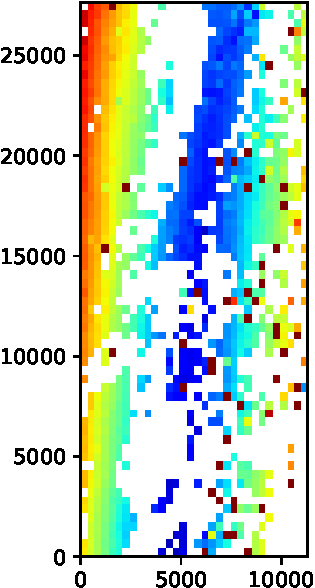
\includegraphics[width=0.8\textwidth]{xcorr-result}
    \end{minipage}
}
\subfloat[xcorr2]{
    \label{fig:exp_xcorr2_result}
    \begin{minipage}[t]{0.30\textwidth}
        \centering
        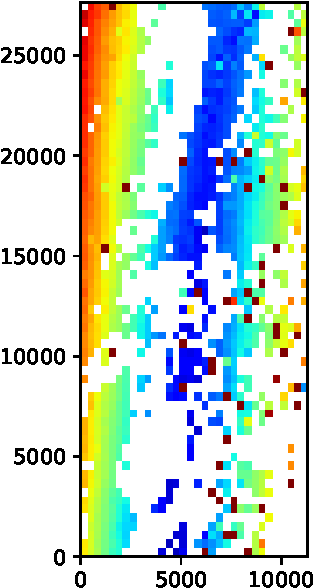
\includegraphics[width=0.8\textwidth]{xcorr2-result}
    \end{minipage}
}
\subfloat[偏移矢量差值]{
    \label{fig:exp_diff_result}
    \begin{minipage}[t]{0.39\textwidth}
        \centering
        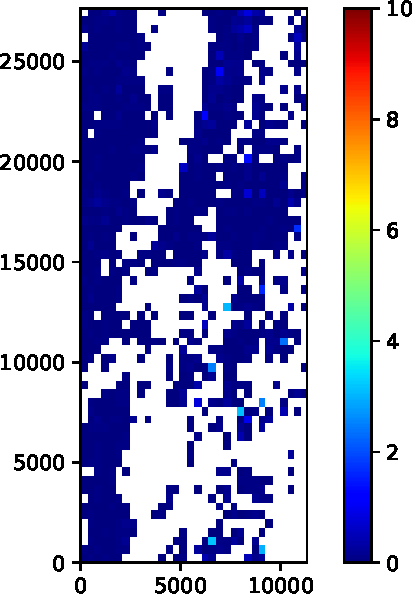
\includegraphics[width=0.8\textwidth]{diff-result}
    \end{minipage}
}
\caption{GMTSAR xcorr 与 xcorr2 配准结果对比} \label{fig:exp_result}
\note{\small 仅包含精配准偏移量。图中仅显示了偏移矢量长度,单位为像素。\\白色部分采样窗口最大互相关小于 GMTSAR aligh.csh 设定的最低值 18,因互相关性太差被筛除。}
\end{figure}

配准后 SLC 图像的相干性(公式 \ref{eq:coherence})是衡量配准精度的重要标准。图 \ref{fig:coh-two} 展示了分别经过 xcorr 和 xcorr2 配准后的主、副 SLC 图像相干性分布图,图 \ref{fig:coh-diff} 显示了相干性分布的差异。图像左下角部分,xcorr2 配准后的相干性略优,而左上角部分则反之。总体上看,相干性差异小于 $3 \times 10^{-3}$,几乎是可以忽略的。

\begin{figure}[htbp]
\centering
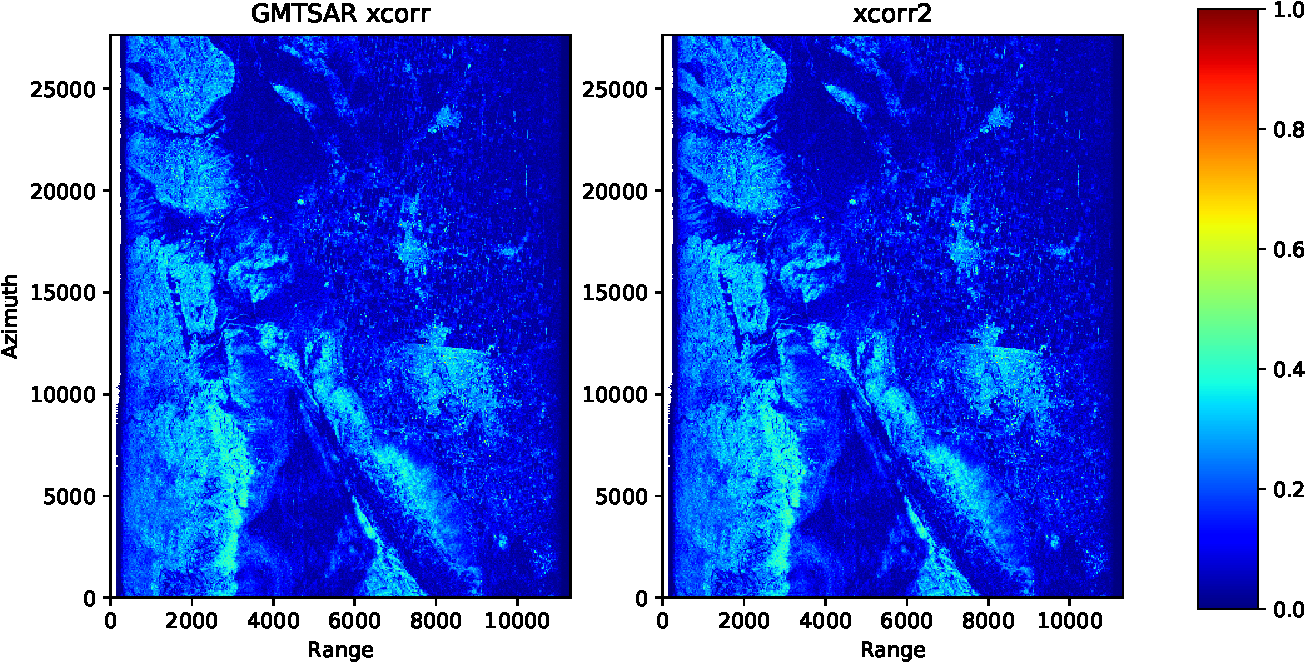
\includegraphics[width=0.85\textwidth]{coh-two}
\caption{配准后 SLC 图像相干性分布图} \label{fig:coh-two}
\note{\small 计算相干性时取像素周围 $8 \times 4$ 像素的邻域}
\end{figure}


\begin{figure}[htbp]
\centering
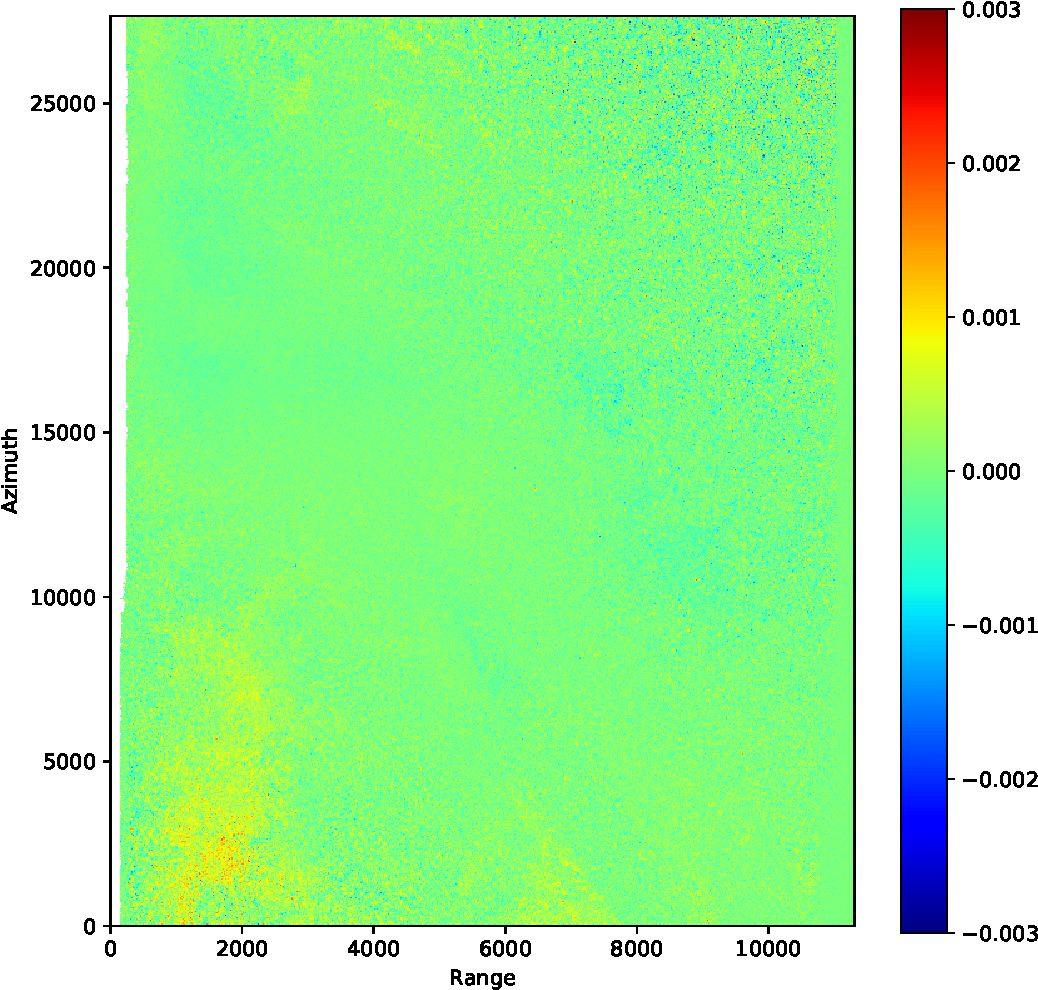
\includegraphics[width=0.60\textwidth]{coh-diff}
\caption{两幅相干性分布图的差值} \label{fig:coh-diff}
\note{\small 用 xcorr2 的计算结果减去 GMTSAR xcorr 的结果}
\end{figure}
